    \subsection{Water balance (JJ)}

    The SMODERP2D episodic rainfall-runoff/erosion model was used for the
    investigation presented here. The 2D model is based on a 1D profile version, in
    which the surface runoff and the erosion were typically calculated in several
    1D profiles representing the main flow path in the hillslope \cite{Dostal2000}.
    The current generation of the SMODERP2D model is pixel distributed, and is
    implemented in python in order to be compatible with most GIS software. The
    development is presented on the github platform at
    \href{https://github.com/storm-fsv-cvut/smoderp2d}{github.com/storm-fsv-cvut/smoderp2d}.

    The SMODERP2D model is primarily designed for surface runoff and erosion
    computation. The surface flow routing in the model is based on the digital
    elevation model (DEM). DEM also controls the spatial discretization of the
    model. The principle of the model is the cell-by-cell mass balance calculated
    in each time step. The change in the water level of the shear flow in any cell
    in time is controlled using the equation: 
    \begin{equation} 
    \frac{\mathrm{d}h}{\mathrm{d}t} = es_{i,t-1} + q^{in}_{i,t-1} - inf_{i,t-1} - q^{out}_{i,t-1},
    \label{eq:bilance}
    \end{equation}
    where h is the surface water level (L), qin and qout are the sheet overland
    inflow and outflow into and out of a given raster cell ($\mathrm{L.t^{-1}}$),
    ep is the effective precipitation intensity (the potential precipitation
    reduced by the interception zone and the surface retention)
    ($\mathrm{L.t^{-1}}$), and inf is the infiltration rate ($\mathrm{L.t^{-1}}$).


    %The principle of the model is the cell-by-cell mass balance calculated in each
    %time step. The change in the water level of the shear flow in any cell in time
    %is controlled using the equation:  
    %
    %[Equation] 
    %	
    %(1) 
    %
    %where h is the surface water level (L), qin and qout are the sheet overland
    %inflow and outflow into and out of a given raster cell (L.t−1), ep is the
    %effective precipitation intensity (the potential precipitation reduced by the
    %interception zone and the surface retention) (L.t−1), and inf is the
    %infiltration rate (L.t−1).  
    %
    %The SMODERP2D model is subjected to uniform rainfall. The potential
    %precipitation is reduced due to surface retention. The surface retention is the
    %storage that needs to be filled before surface runoff can occur.  
    %
    %The time derivative in Equation (1) is calculated using an explicit method. The
    %computation is therefore sensitive to the size of the time step. The size of
    %the time step is controlled by the Courant criterion, which needs to be kept
    %below the theoretical maximum value of 1, while the maximum value in practise
    %is lower than 1 [46,47].  
    %
    %The sheet flow water level of the next time t + 1 step in Equation (1) which
    %incorporates the sum (5) is calculated with the explicit time discretisation
    %scheme for cell i as: 
    %
    %[Equation] 
    %	
    %(6) 

        \subsubsection{Interception component (JJ)}
            The SMODERP2D model is subjected to uniform potential rainfall
            $ps$.  The potential precipitation is reduced due to vegetation
            interception to effective precipitation.  To calculated the
            effective  precipitation the potential interception (amount of
            water stored on vegetation) and canopy cover (percentage of surface
            covered by vegetation) needs to be provided.  For time $t$ the
            effective precipitation is calculated as:
            $$
            es_t= 
              \begin{cases}
              ps_t(1 - cc),& \text{if} \sum_{\bar{t} = t_{init}}^{t} (ps_{\bar{t}} cc) <= pi\\
              {ps}_t,             & \text{else}
            \end{cases}
            $$
            where $ps$ is potential precipitation, $cc$ canopy cover, and is
            $pi$ potential precipitation.  The sum $\sum_{\bar{t} =
            t_{init}}^{t} (ps_{\bar{t}} cc) <= pi$ indicated the amount of
            water that accumulated in the interception zone from the initial
            time to the current computation time.
            
        \subsubsection{Infiltration component (JJ) }
            The infiltration component of Equation \ref{eq:bilance} is calculated by the
            Philip infiltration equation \citep{philip1957}
            \begin{equation} 
            inf = \frac{1}{2}St^{-1/2}+K_s.
            \label{eq:infiltration}
            \end{equation} 
            where S stands for sorptivity ($\mathrm{L.t^{1/2}}$) and ($\mathrm{K_s}$)
            stands for saturation hydraulic conductivity ($\mathrm{L.t^{-1}}$).

            {\bf GA}
 
            %Phillip infiltration 
            %
            %The infiltration component of Equation (1) is calculated by the
            %Philip infiltration equation [44] 
            %
            %[Equation], 
            %	
            %
            %(4) 
            %
            %where S stands for sorptivity (L.t1/2) and Ks stands for
            %saturation hydraulic conductivity (L.t−1). 
            %
            %GA??? 

 

        \subsubsection{Surface retention component (JJ)}
    \subsection{Sheet flow hydraulics (JJ)}
        The kinematic wave approach is used in the calculation of the overland flow.
        The momentum is therefore expressed by the power-law:

        \begin{equation} 
        q = ah^b
        \label{eq:powerlaw}
        \end{equation}
        where a and b are power-law parameters. Equation \ref{eq:powerlaw} can be
        expressed in the form of the Manning–Strickler formula


        \begin{equation} 
        q = n^{-1} s^Y h^b,
        \label{eq:powerlaw2}
        \end{equation}
        where n is roughness,  Y  empirical parameter and s is the surface
        slope ($\mathrm{L.L^{-1}}$).
        \subsubsection{Principle of the solution}

             %The kinematic wave approach is used in the calculation of the
             %overland flow. The momentum is therefore expressed by the power-law: 
             %
             %[Equation], 
             %	
             %
             %(2) 
             %
             %where a and b are power-law parameters. Equation (2) can be
             %expressed in the form of the Manning–Strickler formula 
             %
             %[Equation] 
             %	
             %
             %(3) 
             %
             %where b and Y are empirical parameters and s is the surface slope
             %(L.L−1). n- Manning roughness coefficient for sheet flow 
             %
             % 
             %
             %XXX -  tables here or link to user guide 

        \subsubsection{D8/ Multiple flow approach}

            The flow routing of the surface runoff is based on the D8 one-direction flow
            algorithm \cite{o1984extraction}. The inflow to cell i is defined as the sum of the sheet
            outflows from the adjacent cells, as:

            \begin{equation} 
            q^{in}_{i,t-1} = \sum_j^m q^{out}_{j,t-1}, 
            \label{eq:d8}
            \end{equation} 
            where j is the index of the adjacent up-slope cells identified by the D8 flow
            algorithm.

            %Two (optional) types of flow direction can be used in the model solution 
            %
            %D8 algorithm 
            %
            %The flow routing of the surface runoff is based on the D8
            %one-direction flow algorithm [45]. The inflow to cell i is defined
            %as the sum of the sheet outflows from the adjacent cells, as: 
            %
            %[Equation], 
            %	
            %
            %(5) 
            %
            %where j is the index of the adjacent up-slope cells identified by
            %the D8 flow algorithm. 
            %
            %Multiple flouw algorithm 
            %
 

        \subsection{Rill flow formation and hydraulics (JJ)}

            %For each soil type a critical value of the tangential stress and velocity was
            %estimated. From this critical value critical height in each cell is calculated.
            %In principle this is a comparison of the current level and its critical value
            %at each time interval. If the critical value is exceeded, the calculation
            %enters the stage at which the rill starts to form. Dimensions of the rills are
            %calculated from volume of the water exceeding the critical value. Sheet surface
            %runoff is then calculated using the critical value level instead of current
            %height in the time step. Once the level has dropped below the critical height
            %value, the calculation returns only in the calculation of surface runoff. The
            %resulting rasters of rill flow and speed in the rill are stored in
            %user-selected directory along with vector shapefile of created rills.
            %Calculation of the flow in the rill is based on Manning equation. 

        \subsubsection{Rill formation (JJ)}

            The rill flow is also included in the calculation. In SMODERP2D, rill flow in a
            cell occurs if $h>h_{crit}$, where $h_{crit}$ is the critical water level. The
            water flow corresponding to the water level above the critical water level has
            enough energy to start to carry the soil particles and to create a rill.

            The critical water level $h_{crit}$ is calculated as:
            \begin{equation}
              h_{crit} = MIN(h_{v_{crit}},h_{\tau_{crit}}),
              \label{eq:critdef}
            \end{equation}
            where $h_{v_{crit}}$ is the water corresponding to the critical velocity, and
            $h_{\tau_{crit}}$ is the water level corresponding to the critical shear
            stress.  As shown in Formula \ref{eq:critdef}, $h_{crit}$ uses several values
            obtained with a different approach. This approach is adopted in order to remain
            on the safe side of the emergence of a rill, since $h_{v_{crit}}$ is more
            sensitive to the sheet flow velocity and $h_{\tau_{crit}}$ is more sensitive to
            the slope of the soil surface. 

            When the condition $h>h_{crit}$ is fulfilled, a rill starts to develop in a
            given cell and $h_{sheet}=h_{crit}$. In SMODERP2D, the rill is a dynamic component and
            can increase as the rill flow increases. The rill volume is controlled by the
            volume of water corresponding to the rill water level $h_{rill}$. This volume is
            calculated as:


            \begin{equation}
              V_{rill} = h_{rill}P,
              \label{eq:rillvol}
            \end{equation}

            The critical water level $h_{crit}$ is calculated as:
            \begin{equation}
              h_{rill} = MAX(h-h_{crit},0),
              \label{eq:hrill}
            \end{equation}
            P stands for the size of the raster cell. 
            %The rill flow is also included in the calculation. In SMODERP2D, rill flow in a
            %cell occurs if [Equation], where [Equation] is the critical water level. The
            %water flow corresponding to the water level above the critical water level has
            %enough energy to start to carry the soil particles and to create a rill. 
            %
            %The critical water level [Equation] is calculated as: 
            %
            %[Equation] 
            %	
            %
            %(7) 
            %
            %where [Equation] is the water corresponding to the critical velocity, and
            %[Equation] is the water level corresponding to the critical shear stress. As
            %shown in Formula (7), [Equation] uses several values obtained with a different
            %approach. This approach is adopted in order to remain on the safe side of the
            %emergence of a rill, since [Equation] is more sensitive to the sheet flow
            %velocity and [Equation] is more sensitive to the slope of the soil surface.  
            %
            %When the condition [Equation] is fulfilled, a rill starts to develop in a given
            %cell and [Equation]. In SMODERP2D, the rill is a dynamic component and can
            %increase as the rill flow increases. The rill volume is controlled by the
            %volume of water corresponding to the rill water level [Equation] This volume is
            %calculated as: 
            %
            %[Equation] 
            %	
            %
            %(8) 
            %
            %where: 
            %
            %[Equation] 
            %	
            %
            %(9) 
            %
            %P stands for the size of the raster cell. 

        \subsubsection{Rill hydraulics (JJ)}\label{sec:rill}

            The rill is simplified as a small channel at the soil surface with
            a rectangular cross section. The rectangle has width $b_{rill}$ and
            rill height $y_{rill} = 0.7b_{rill}$. The rill flow is as
            calculated with the Manning equation: 

            \begin{equation}
                q_{rill} = \frac{A}{n_{rill}} s^{1/2} R_{rill}^{2/3},
              \label{eq:rillflow}
            \end{equation}
            where A is the cross section of the rill,  $n_{rill}$ is the roughness in the
            rill, s is the surface slope, and  $R_{rill}$  is the hydraulic radius of the
            rill. 

            As stated above, the size of the rill changes as $h_{rill}$ increases. The
            scheme of this change is shown in Figure \ref{fig:rill_plneni}. The change in
            the rill flow varies with the change in $R_{rill}$ in Equation
            \ref{eq:rillflow}, since $h_{rill}$ increases, and therefore $y_{rill}$ and
            $b_{rill}$ also increase. The $R_{rill}$ for an increasing rill is calculated
            as:
            \begin{equation}
                R_{rill} = \frac{h_{rill}b_{rill}}{2h_{rill}+b_{rill}}  =
                \frac{y_{rill}b_{rill}}{2y_{rill}+b_{rill}},
              \label{eq:rrill}
            \end{equation}
            where:
            \begin{equation}
              b_{rill} = h_{rill}/0.7
              \label{eq:brill}
            \end{equation}


            \begin{figure}[b]
                \centering
                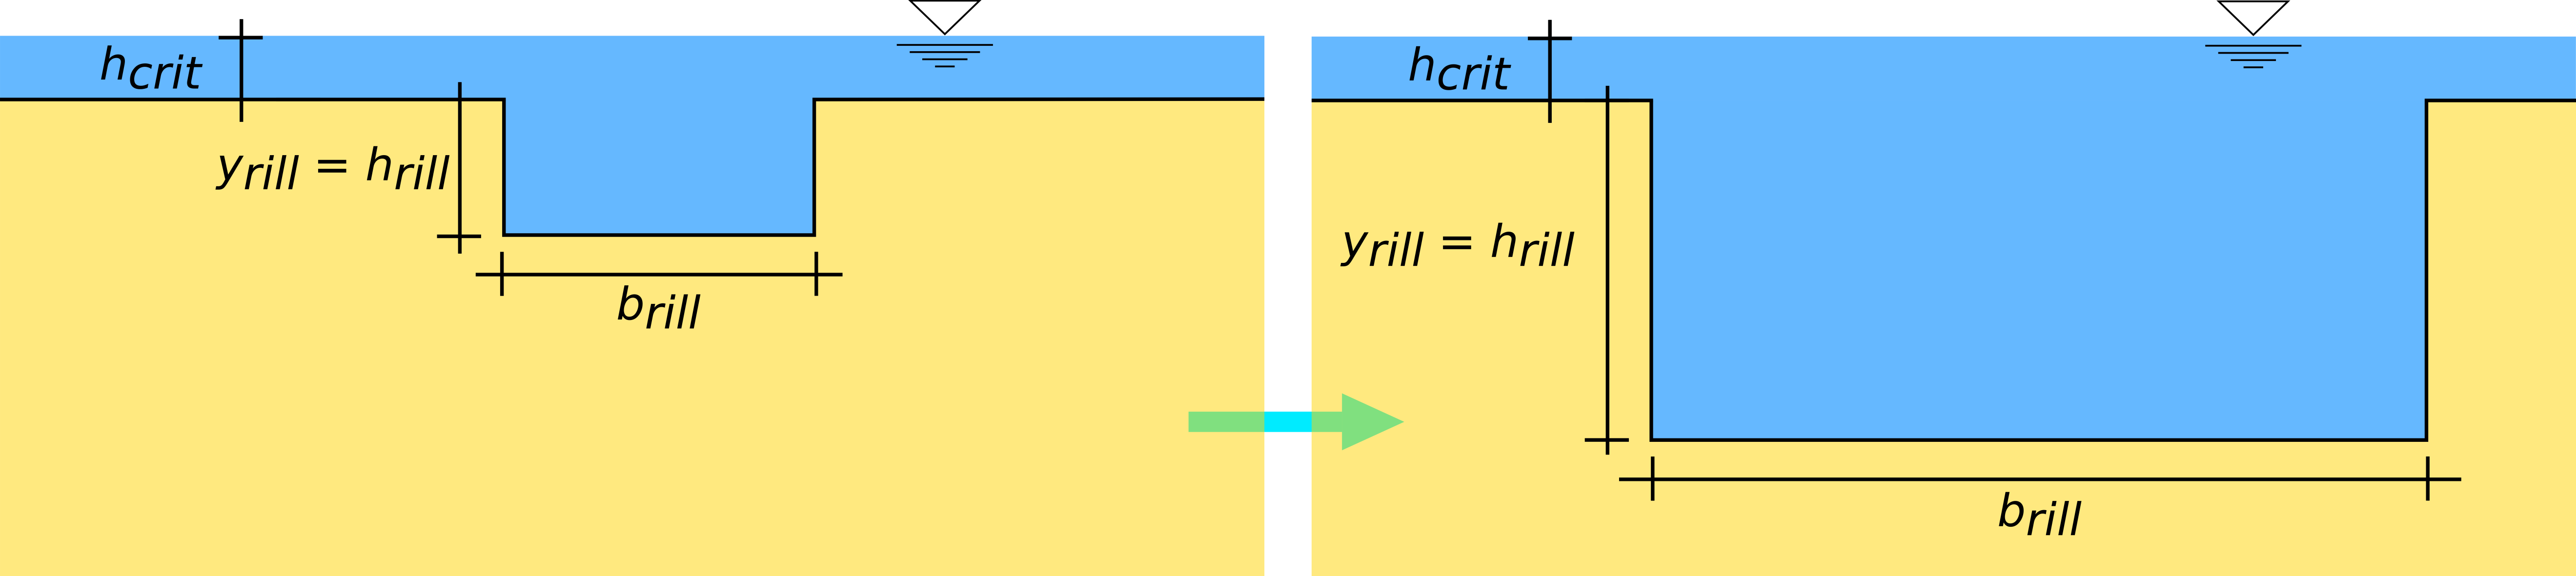
\includegraphics[width=1\linewidth]{./img/rill_schema_plneni.png}
                \caption{Scheme of the rill size during increasing surface runoff.}
                \label{fig:rill_plneni}
            \end{figure}


            During the recession limb of the hydrograph, the rill size “locks”, and
            $h_{rill}$ decreases until the rill is empty. The scheme of the emptying rill
            and the rill flow is shown in Figure~\ref{fig:rill_prazdneni}. In this case,
            $R_{rill}$ is calculated from fixed $b_{rill}$ and decreasing $h_{rill}$.
            $R_{rill}$ for decreasing rill flow is calculated as:
            \begin{equation}
                R_{rill} = \frac{h_{rill}b_{rill}}{2h_{rill}+b_{rill}},
              \label{eq:rrill2}
            \end{equation}
            where:
            \begin{equation}
              b_{rill} = y_{rill}/0.7
              \label{eq:brill2}
            \end{equation}

            \begin{figure}[t]
                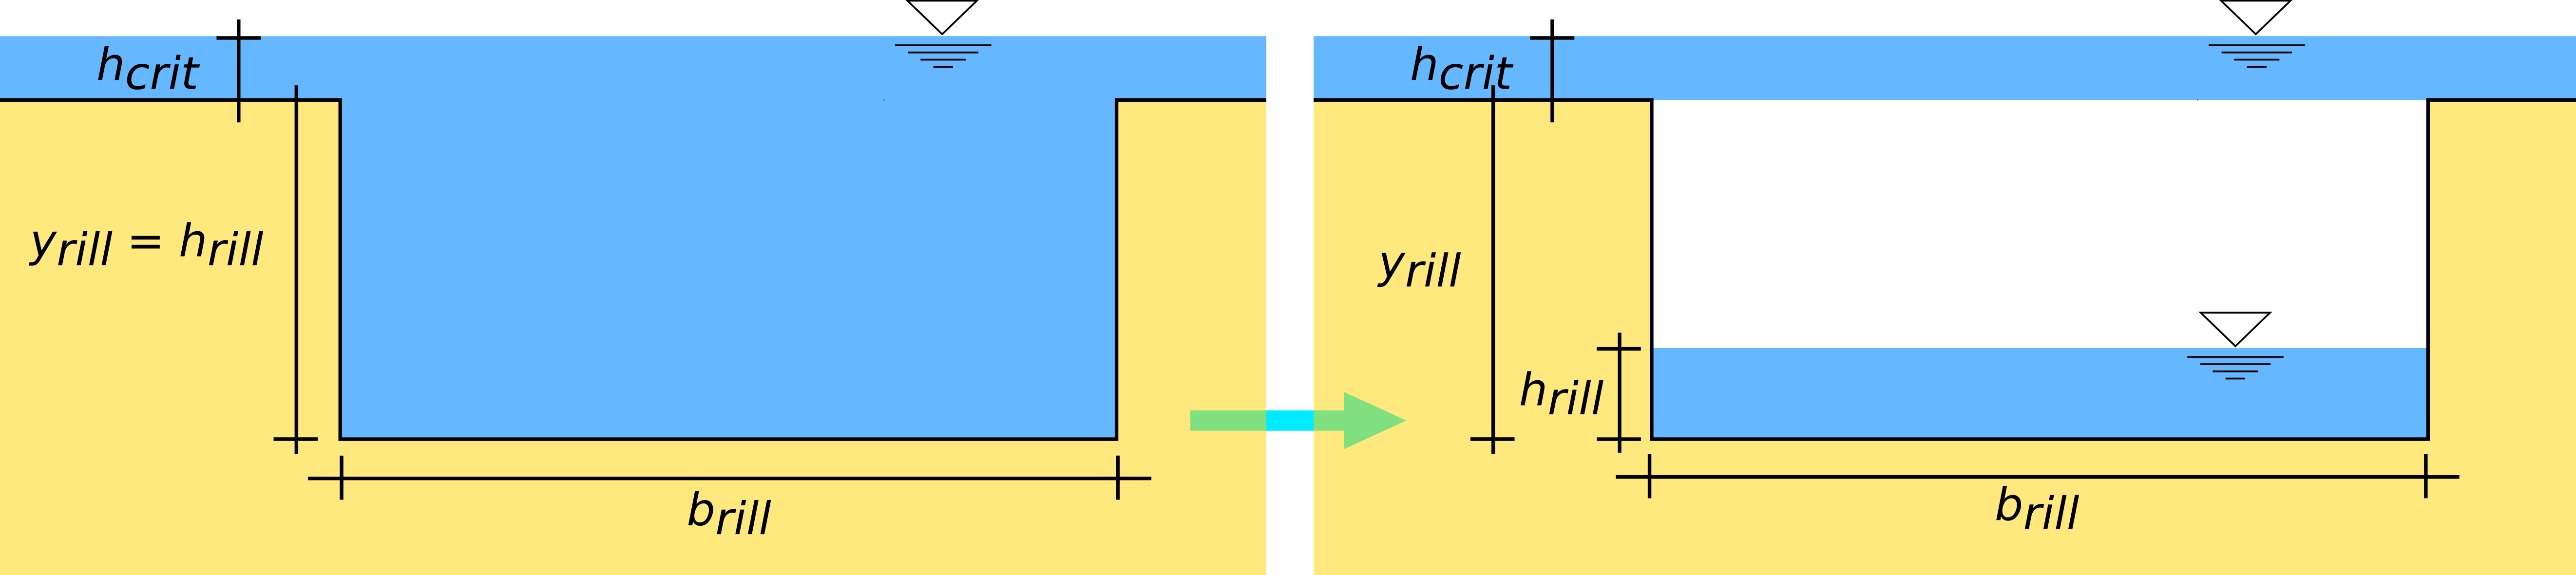
\includegraphics[width=1\linewidth]{./img/rill_schema_prazdneni.png}
                \caption{Scheme of the rill size during the recession limb of the hydrograph.}
                \label{fig:rill_prazdneni}
            \end{figure}

            The total water balance in cell i, where a rill is developed, is calculated as:

            \begin{equation}
                \frac{\mathrm{d}h_i}{\mathrm{d}t} = es_i + q^{in}_{sheet,i}(h_{sheet,i})
                +q^{in}_{rill,i}(h_{rill,i}) - (inf_i + q^{out}_{sheet,i}(h_{sheet,i}) +
                q^{out}_{rill,i}(h_{rill,i}))
                %
                %
                %h_{i,t} =h_{i,t} + \mathrm{d}t (es_{i,t-1} + \sum_j^m q^{out}_{j,t-1}-
                %inf_{i,t-1} - q^{out}_{i,t-1}),
            \end{equation}
            where:
            \begin{equation}
                q^{in}_{sheet,i} = \sum_j^m q^{out}_{sheet, j}(h_{sheet,j}),\quad \mathrm{and}
            \end{equation}
            \begin{equation}
                q^{in}_{rill,i} = \sum_j^m q^{out}_{rill, j}(h_{rill,j})
            \end{equation}

            and:
            \begin{equation}
               h = h_{rill} + h_{sheet}  
            \end{equation}

            The rill water level is recalculated to cover the whole cell and not just the
            bottom of the rill, as shown in Figures \ref{fig:rill_plneni} and
            \ref{fig:rill_prazdneni}.
            %The rill is simplified as a small channel at the soil surface with a
            %rectangular cross section. The rectangle has width[Equation] and rill height
            %[Equation]. The rill flow is as calculated with the Manning equation:  
            %
            %[Equation] 
            %	
            %
            %(10) 
            %
            %where A is the cross section of the rill, [Equation] is the
            %roughness in the rill, s is the surface slope, and [Equation] is the
            %hydraulic radius of the rill.  
            %
            %As stated above, the size of the rill changes as [Equation] increases. The
            %scheme of this change is shown in Figure 1. The change in the rill flow varies
            %with the change in [Equation] in Equation (10), since [Equation] increases, and
            %therefore [Equation] and [Equation] also increase. The [Equation] for an
            %increasing rill is calculated as: 
            %
            %[Equation] 
            %	
            %
            %(11) 
            %
            %where: 
            %
            %[Equation] 
            %	
            %
            %(12) 
            %
            %  
            %
            %Figure 1. Scheme of the rill size during increasing surface runoff. 
            %
            %During the recession limb of the hydrograph, the rill size
            %“locks”, and [Equation] decreases until the rill is empty. The scheme
            %of the emptying rill and the rill flow is shown in Figure 2. In this
            %case, [Equation] is calculated from fixed [Equation] and decreasing
            %[Equation]. [Equation] for decreasing rill flow is calculated as: 
            %
            %[Equation] 
            %	
            %
            %(13) 
            %
            %where: 
            %
            %[Equation] 
            %	
            %
            %(14) 
            %
            % 
            %
            %Figure 2. Scheme of the rill size during the recession limb of the hydrograph. 
            %
            %The total water balance in cell i, where a rill is developed, is calculated as: 
            %
            %[Equation] 
            %	
            %
            %(15) 
            %
            %where: 
            %
            %[Equation] 
            %	
            %
            %(16) 
            %
            %[Equation] 
            %	
            %
            %(17) 
            %
            % 
            %
            %and: 
            %
            %[Equation] 
            %	
            %
            %(18) 
            %
            % 
            %
            %The rill water level is recalculated to cover the whole cell and not just the bottom of the rill, as shown in Figures 1 and 2. 

 

    \subsection{Kinematic / Diffuse approach}

        \subsubsection{Kinematic}
        \subsubsection{Diffuse}

    \FloatBarrier
    \subsection{Implicit /Explicit approach}

        \subsubsection{Explicit}
            The time derivative in Equation \ref{eq:bilance} is calculated using an
            explicit method. The computation is therefore sensitive to the size of the time
            step. The size of the time step is controlled by the Courant criterion, which
            needs to be kept below the theoretical maximum value of 1, while the maximum
            value in practise is lower than 1 
            \cite{zhang1989modeling, esteves2000overland}.


            The sheet flow water level of the next time t + 1 step in Equation
            \ref{eq:bilance} which incorporates the sum \ref{eq:d8} is calculated with the
            explicit time discretisation scheme for cell i as:
            \begin{equation} 
            h_{i,t} =h_{i,t-1} + \mathrm{d}t (es_{i,t-1} + \sum_j^m q^{out}_{j,t-1}-
            inf_{i,t-1} - q^{out}_{i,t-1}),
            \label{eq:bilanceexpl}
            \end{equation}


           After inserting the equations~(\ref{eq:infiltration})
           and~(\ref{eq:powerlaw2}) into equation~(\ref{eq:bilanceexpl}) the
           final explicit form balance equation can be written as:
            \begin{dmath}
              h_{i,t} = h_{i,t-1} +
              es_{i,t-1}  + exf_{i,t-1} +  \sum_{j}^{inflows}
              1/n_{sheet,j}I_j^{y_j} h_{j,t-1}^{b_j} -
              1/n_{sheet,i}I_i^{y_i}h_{i,t-1}^{b_i} - ( 
              \frac{1}{2}S_it_1^{-1/2}+K_{s,i}).
            \end{dmath}


        \subsubsection{Implicit}
        Alternatively the equation (\ref{eq:bilance}) solved using implicit
        scheme. The right hand side can be expressed in for time $t$ as:

        $$
          \frac{h_{i,t} - h_{i,t-1} }{\mathrm{d} t} =  \left(es_{i,t} +
          \sum_j^{inflows} q^{in}_{j,t} - inf_{i,t} - q^{out}_{i,t}\right).
        $$

        After inserting the power-law equation (\ref{eq:powerlaw}) and several rearrangements the formula above can be written 
        as follows: 



        $$
          h_{i,t} + \mathrm{d} t a_ih^{b_{i}-1}_{i,t} h_{i,t} - \mathrm{d} t \sum_j^{inflows}
          a_jh^{b_{j}-1}_{j,t} h_{j,t} = h_{i,t-1} + \mathrm{d} t es_{i,t} - \mathrm{d}
          t inf_{i,t}.
        $$
        Here the known part of the balance equation (rainfall and infiltration) are at the right hand side. To 
        extract the unknown $h$ form the power law a following rearrangement was used:



        \begin{equation}
          (1+\mathrm{d} t a_ih^{b_{i}-1}_{i,t})h_{i,t} - \mathrm{d} t \sum_j^{inflows}
          a_jh^{b_{j}-1}_{j,t} h_{j,t} = h_{i,t-1} + \mathrm{d} t es_{i,t} -
          \mathrm{d} t inf_{i,t}
          \label{eq:impl}
        \end{equation}

        From the equation (\ref{eq:impl}) the system of linear equations can be constructed. 

        As example, lets show the equation (\ref{eq:impl}) for
        $
        i=5\ \mathrm{and}\ inflows\in\{7,8,9\}
        $:


        \begin{dmath}
          (1+\Delta T a_5h^{b_{5}-1}_{5,t})h_{5,t} - \Delta T a_7h^{b_{7}-1}_{7,t} h_{7,t} + \Delta T a_8h^{b_{8}-1}_{8,t} h_{8,t} + \Delta T a_9 h^{b_{9}-1}_{9,t} h_{9,t}  = h_{5,t-1} + \Delta T es_{5,t} - \Delta T inf_{5,t}.
        \end{dmath}

        In matrix form the above equation can be written as:



        \begin{dmath}
        \begin{bmatrix}
        \hdots& & & & & &  \\
        \hdots  & 1+\Delta T a_5h^{b_{5}-1}_{5,t} & \hdots &  \Delta T a_7h^{b_{7}-1}_{7,t} &  \Delta T a_8h^{b_{8}-1}_{8,t} & \Delta T a_9 h^{b_{9}-1}_{9,t} & \hdots \\
        \hdots&  & & & & &  \\
        \hdots& && &  &  & \\
        \hdots& && &  &   & \\
        \hdots& && &  &   & \\

        \end{bmatrix} 
        % 
        \begin{bmatrix}
         \vdots \\
         h_{5,t} \\
         \vdots \\
         h_{7,t} \\
         h_{8,t} \\
         h_{9,t} \\
         \vdots \\
        %  
        \end{bmatrix}
        =
        \begin{bmatrix}
         \vdots \\
        h_{5,t-1} + \Delta T es_{5,t} - \Delta T inf_{5,t} \\
         \vdots \\
         \vdots \\
         \vdots \\
         \vdots \\
         \vdots \\
        %  
        \end{bmatrix}
        \label{eq:sys}
        \end{dmath}

        The system (\ref{eq:sys}) is solved using \texttt{scipy} package method \texttt{root}
        using \texttt{krigov} methof that shown the best convergence.


        \paragraph{Implicit solution with rill flow} To calculated rill flow the water level in rill and needs to be calculated as 
        \begin{equation}
        h_{rill} = \text{max}(h-h_{crit},0),
            \label{eq:hrill2}
        \end{equation}
        where 
        \begin{equation}
        h_{sheet} = \text{min}(h,h_{crit}).
            \label{eq:hsheet2}
        \end{equation}

        Mannings formula is used to calculated the steady state flow in
        the rill assuming rill is a channel (description in section \ref{sec:rill}.  
        $$
        q_{rill} = 1/n R(h_{rill})^{2/3} i^{1/2}
        $$


        The balance equation becomes
        \begin{dmath}
          \frac{h_{i,t} - h_{i,t-1} }{\Delta T} = 
          es_{i,t} + \sum_j^{inflows} a_jh^{b_{j}}_{sh,j,t}  + \sum_k^{inflows} 1/n_k R_k(h_{rl,k,t})^{2/3} i_k^{1/2} - inf_{i,t} - a_ih^{b_{i}}_{sh,i,t} - 1/n R(h_{rl,i,t})^{2/3} i^{1/2},
        \end{dmath}
        where $h_{sheet}$ and $h_{rill}$ are defined as (\ref{eq:hsheet2}) and  (\ref{eq:hrill2}).

        This formula is rearranged and, for practical purposes, the linear equation is the system is calculated with condition \\
        for  $h<=h_{crit}$ as
        \begin{equation}
            \left(\frac{1}{\Delta T}+a_ih^{b_{i}-1}_{i,t}\right)h_{i,t} -  \sum_j^{inflows} a_jh^{b_{j}-1}_{j,t} h_{j,t} = \frac{h_{i,t-1}}{\Delta} +  es_{i,t} - inf_{i,t}
        \end{equation}
        % 
        % 
        and for  $h>h_{crit}$ as
        \begin{multline}
          \left(\frac{1}{\Delta T}
          + 1/n_i R_i(h_{i,t}-h_{crit,i})^{2/3} i_i^{1/2} \frac{1}{h_{i,t}}\right)h_{i,t} \\
            - \sum_k^{inflows} \left( 1/n_k R_k(h_{k,t}-h_{crit,k})^{2/3} i_k^{1/2}  \frac{1}{h_{k,t}}\right)h_{k,t}
          =  \\
          \frac{h_{i,t-1} }{\Delta T}
          + es_{i,t} 
          + \sum_j^{inflows} a_j h^{b_{j}}_{crit,j}  
          - inf_{i,t} 
          - a_i h^{b_{i}}_{crit,i} 
        \end{multline}
    The later system of equations is constructed in similar fashion as the case of (\ref{eq:sys}) and solved with the same solver.


    \FloatBarrier
    \subsection{Input data requirements and description}

        \begin{table}%[!htp]
  \centering
    \caption{Overview of soil type and land use parameters}
    \begin{tabular}{p{3.8cm}l}
    \hline  \hline
        symbol in input table (format mandatory) & description of parameter and unit \\
    \hline
        k&  soil hydraulic conductivity [m/s]\\
        s&  soil sorptivity [$\mathrm{m/s^{1/2}}$]\\
        n&   Mannings surface roughness for sheet flow[-] \\
        b&   power law parameter [-] \\
        y&   power law parameter [-] \\
        nrill&  Mannings surface roughness for rill flow[-] \\
        pi&   potential interception [m]\\
        ppl& canopy cover [-] \\
        ret& surface retention [m] \\
        tau& critical sheer stress [Pa] \\
        v &  critical water velocity [m/s] \\
    \hline  \hline
    \end{tabular}%
  \label{tab:soilveg}%
\end{table}%

        \subsubsection{DMR}
        \subsubsection{Soil}
        \subsubsection{Land Use}
        \subsubsection{Soil and Land Use  combination}
            \begin{figure}[!b]
                \centering
                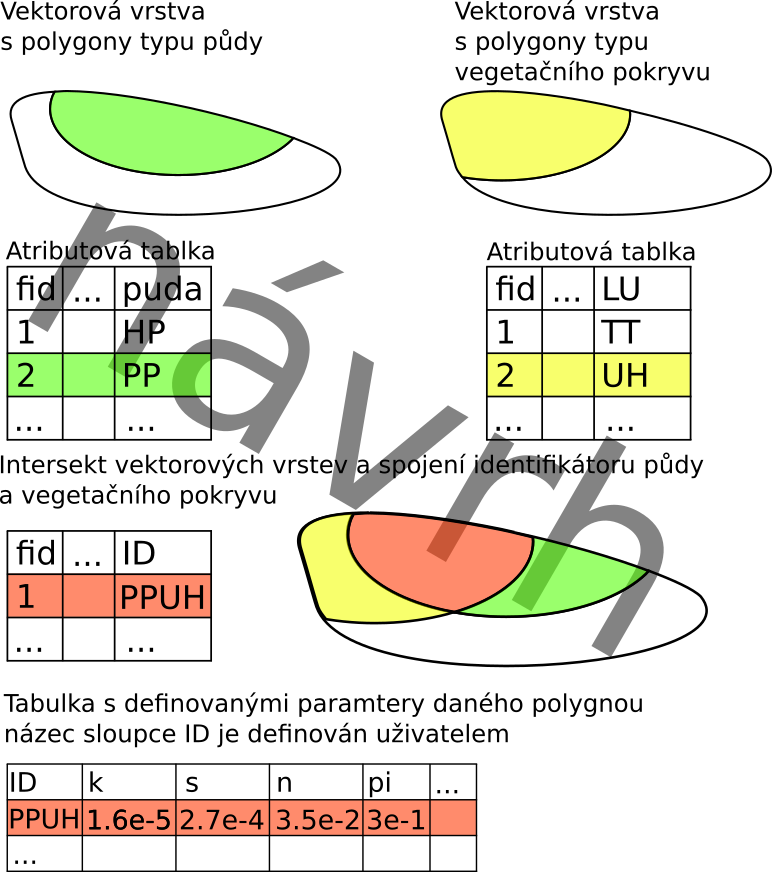
\includegraphics[width=0.5\linewidth]{./img-prep/spojenistabulkou.png}
                \caption{Combination of soil and landuse characteristics}
                \label{fig:soilvegcreate}
            \end{figure}
        





